{Use six rectangles to approximate the area under the given graph of $f$ from $x=0$ to $x=12$, using:
\begin{enumerate}
\item The Left Hand Rule,
\item The Right Hand Rule,
\item The Midpoint Rule.
\end{enumerate}
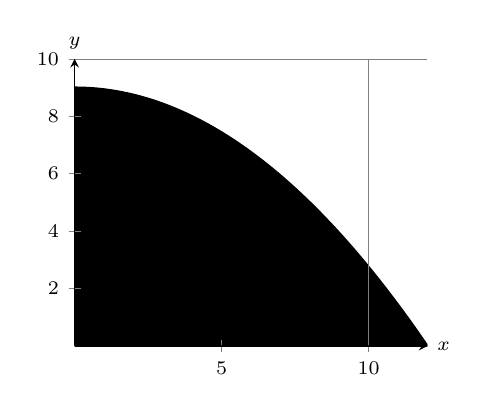
\begin{tikzpicture}
\begin{axis} [width=.5\textwidth,%\marginparwidth+25pt,
tick label style={font=\scriptsize},axis y line=middle,axis x line=middle,
name=myplot,axis on top,%all axes={grid},
                        ymin=0,ymax=10,
                        xmin=0,xmax=12,smooth]
   \addplot [{\coloronefill},fill={\coloronefill},area style,domain=0:12] {9-(x/4)^2} \closedcycle;
   \addplot [smooth,thick,{\colorone},domain=0:12] {9-(x/4)^2};
   \draw [help lines,step=10] (axis cs:0,0) grid (axis cs:12,10);
   % steps=10 was guess and check
\end{axis}
\node [right] at (myplot.right of origin) {\scriptsize $x$};
\node [above] at (myplot.above origin) {\scriptsize $y$};
\end{tikzpicture}}
{\begin{enumerate}
\item	Exact expressions will vary; $80.5$.
\item	$72.25$
\item	$62.5$
\end{enumerate}}
